% Chapter 1

\chapter{Introduction} % Main chapter title

\label{chapter1} % For referencing the chapter elsewhere, use \ref{Chapter1}

%----------------------------------------------------------------------------------------
\section{Motivation and significance}
A question was posed in 2017: "Will there be a software service for the generation of explanations and arguments in law that will assist in structuring explanations of answers and supportive legal arguments?" (\cite{ashley_2017}). This question seems close to getting an answer in 2023 with the release of ChatGPT (\cite{openai}) to the general public. Consider the following response from ChatGPT:  

\begin{figure}[!ht]
	\centering
	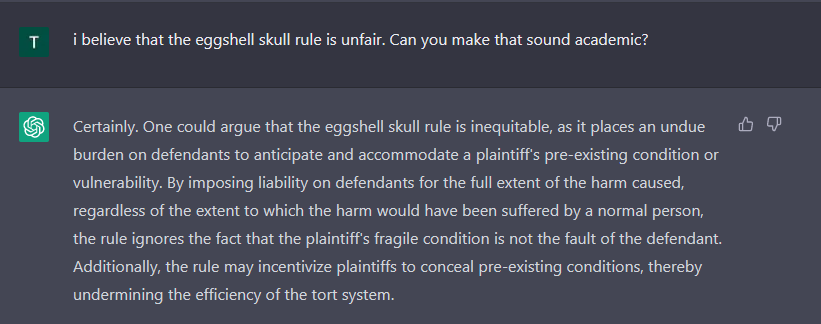
\includegraphics[width=1\linewidth]{figures/chatgpt3.png}
	\caption{Conversation with ChatGPT about the egg-shell skull rule.}   
  \label{fig:chatgpt}
\end{figure}

Indeed, GPT-4, successor of ChatGPT and released a mere 4 months after ChatGPT, scored on the 90th percentile on the Uniform Bar Exam which is significantly in excess of the passing mark to practice law in the US (\cite{katz2023gpt}).

ChatGPT and GPT-4 are the most recent AI models that uses advanced natural language processing (NLP). NLP is a branch of AI that gives computers the ability to understand text and spoken words as how human beings would understand (\cite{ibm_nlp}). While NLP techniques have substantially increased in performance in recent years, it has come at the cost of the explainability of their predictions because of models that are architecturally more complex (\cite{zini2022}). This issue of explainability is exemplified by the last question I posed to ChatGPT about its view on the egg-shell skull rule:

\begin{figure}[!ht]
	\centering
	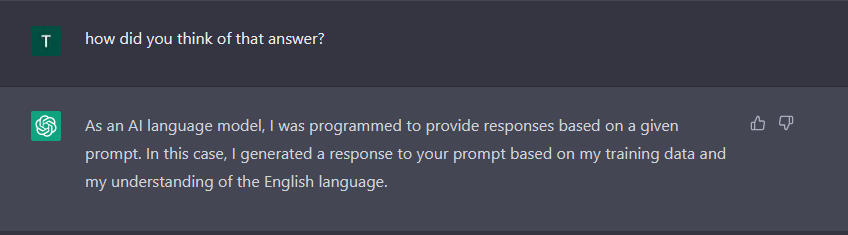
\includegraphics[width=1\linewidth]{figures/chatgpt2.png}
	\caption{Conversation with ChatGPT about the egg-shell skull rule.}   
  \label{fig:chatgpt2}
\end{figure}

ChatGPT does not seem to be able to explain its views like how a typical human would\footnote{Further prompting led ChatGPT to provide a list of academic papers that support its view. But there are issues of hallucination, where ChatGPT generates answers about facts that are false or non-existent (\cite{alkaissi2023}).}. This lack of explainability could be a significant hindrance towards NLP's greater adoption within the legal industry because the lawyer that uses these models ultimately bear the legal responsibility of ensuring that the analysis is legally sound. In Singapore, a legal practitioner must act with reasonable diligence and competence in the provision of services to the client\footnote{According to r5(2)(c) of the Legal Profession (Professional Conduct) Rules 2015.}. A lawyer that relies on the analysis of legal tech tools but does not understand how the analysis was produced could be considered lacking in diligence and competence.

Nevertheless, the intersection in skillset between data science and legal analysis is still nascent and it is unrealistic to expect all legally trained personnel to be trained in data science to the extent required to interpret the predictions of machine learning models without aid. Explainable AI (XAI) techniques and research have been rising in popularity since 2020 (\cite{linardatos2020}) but have not been adopted in legal tech. XAI refers to methods that attempt to help the end user of a model understand how it arrives at its result (\cite{danilevsky2020}). XAI for NLP has been designed to combat issues of opacity by reducing the abstraction of NLP techniques so that end users can understand how the model arrived at a decision. XAI can therefore bridge the gap between the lawyer and the data scientist by using XAI techniques to explain the predictions of legal tech AI models. 

However, there is not much consensus about what "explainable" means. While the general agreed upon goal of XAI is to "completely, accurately and clearly quantify the [model's] logic", there is no consistent use of the terms "explainability", "interpretability" and "transparency" (\cite{danilevsky2020}). Interpretability is sometimes used to describe the model's internal logic and explainability as the ability of the user to understand that logic. Explainability is also sometimes described as techniques to explain the model's logic post-hoc without necessarily being representative of the model's true decision (\cite{rosenfeld2021}). Since a debate on the "correct" definition of explainability is out of the scope of this capstone, I use explainability, interpretability and transparency interchangeably.

Another area of XAI is differentiating what explainability means to different users of the model who have different purposes for the explanations. For example, what could be explainable to data scientists may not be explainable to laypersons. While data scientists may find that more technical details about the model would make the model more explainable, laypersons might be more confused if too many details are provided (\cite{rosenfeld2021}). Therefore, assessing the effectiveness of XAI is highly dependent on the specific context and needs of the users. 

In this capstone, XAI is assessed within the context of data privacy. The widespread collection and use of data by organisations in recent years has led to an increase of regulations governing data privacy, with 145 countries having enacted data protection legislation in 2021 (\cite{gstrein2022}). With more sophisticated regulation comes increased difficulties for organisations to ensure that they are complying with these regulations, and for governments to enforce them. Given that explainability is context and user dependent, the below analysis explains why XAI is important to the three different stakeholders in data privacy: the consumer, organisation and state.

For the consumer, it is uncontroversial that data privacy policies on websites and software are rarely read, and even if they are read, consumers are unlikely to fully understand them because of the use of extensive legalese. The ease of reading data privacy policies was measured to be roughly the same as compared to academic articles such as the Harvard Law Review. The average policy takes 17 minutes to read, and the annual reading time per consumer is more than 400 hours which is more than an hour per day\footnote{Assuming that a consumer visits 1462 unique websites each year.} (\cite{wagner2022privacy}). This increasing unreadability of data privacy policies poses a significant challenge to the effectiveness of data privacy regulation given that the current model of regulation depends on the consumer giving consent that is informed and freely given (\cite{mantelero_2014}). Combined with the increasing collection and use of data by organisations, consumers have diminishing control over how their data is collected and used. Therefore, XAI could be helpful to consumers since XAI can be used to automate legal analysis of data privacy policies and explain the implications of the analysis in simple terms.

Organisations in the EU are subjected to a data subject's "right to explanation" under the General Data Protection Regulation (GDPR). Data subjects have the right to obtain an explanation of a decision reached solely through automated processing\footnote{This is a plausible interpretation when reading Recital 71 in conjunction with Art 22 of the GDPR.}. For example, a bank could use AI to predict the probability of a customer defaulting on a loan. This prediction could be used to justify a decision to deny a loan to the customer. Under the GDPR, the customer has the right to not be subjected to such automated processing and obtain an explanation as to why the model made such a prediction. Therefore, the use of opaque AI could potentially affect the organisation meeting their legal obligations.

In Singapore, as part of Personal Data Protection Commission's (PDPC) guidance on the operations management of AI models, organisations are advised to provide explanations on how AI models are incorporated into the decision making process of the organisations so as to build understanding and trust with those stakeholders that use their products (\cite{ai_modelframework}). In terms of communications with their stakeholders, organisations are advised to develop policies on the type of explanations and when to provide them. Such communication could include explanations as to how the AI model was used in a specific decision. 

Despite debate about the scope of the right to explanation and whether it is binding, (\cite{chesterman2021_transparency}), such legislation in addition to the PDPC's guidance for explainability supports the need for further development of XAI specifically in the context of data privacy. The models in this capstone can support the adoption of AI in organisations by providing explanations so as to aid the organisations in checking whether their privacy policies are in compliance with data privacy regulations.

One of the state's concerns when AI is used in legal decision making is the integrity of the judicial system and regulatory activities (\cite{chesterman2021_opacity}) since the legal system depends as much on the justification of its decisions as it does on the decisions themselves. In the context of Singapore's Personal Data Protection Act (PDPA), there is an appeal process for cases appearing before the PDPC and the higher courts can overturn the PDPC's decisions\footnote{Per s48Q, s48R and s54 of the PDPA.}. However, when overturning the PDPC's decisions, the higher courts do not disagree with the outcome but they disagree with the reasoning of the PDPC's decision. Assuming that AI models are sophisticated enough to write (or at least assist the writing) court judgements, if there was no explanation of the model's writing, there would be little basis for the higher courts to overturn judgements made by lower courts. 

Hence, the importance of XAI applies across all three stakeholders in data privacy. Consumers can benefit from XAI by making privacy policies more readable. Organisations can use XAI to be more accountable to consumers and regulators by providing explanations for automated decisions. Transparency brought by XAI also helps the state to regulate organisations' use of AI.

\section{Research questions and roadmap}
Therefore, I focus on NLP and XAI in the specific context of data privacy, as this context provides a realistic and practical scope for evaluating the explainability of AI models\footnote{All code and analysis used in this capstone can be found at \url{https://github.com/TristanKoh/capstone-repo/}.}. To this end, I have four research questions: 

\begin{enumerate}
  \item Which AI classifiers perform the best on a data privacy dataset in terms of traditional performance metrics?
  \item Which classifiers are the most explainable to users that include laypersons and users with domain knowledge in data science and the law?
  \item How would users rate the explainability of a selected XAI technique?
  \item What are the differences in explainability if users were asked to consider the predictions of these classifiers from the perspective of a consumer, an organisation or the PDPC (as the regulatory authority for data privacy)?
\end{enumerate}

To investigate these questions, I train and evaluate the performance of AI models that are able to identify data privacy practices in apps' data privacy policies. A privacy practice describes a certain behaviour of an app that can have privacy implications\footnote{This will be further elaborated on when \hyperref[app350_corpus]{the dataset} is introduced.}. XAI methods are then used to visualise why the models made such predictions, and are assessed for effectiveness by conducting a survey asking respondents to rate these visualisations according to certain metrics related to explainability.

This capstone's objectives come broadly within the evaluation of XAI techniques. While there are studies that evaluate XAI and non-empirical research that investigates the relevant standard for explainability across different areas of law, I adopt an uniquely empirical methodology to assess XAI within a data privacy context across the different use cases of stakeholders. The closest study using similar methodology is one that asked lawyers to rate visualisations generated by different XAI methods (\cite{gorski2021}). However, this study was conducted within the context of the US Board of Veterans' Appeals, and did not consider evaluating explainability from different use cases.

Chapter~\ref{chapter2} introduces the dataset and provides a literature review and methodology of the selected NLP models, XAI techniques, and methods used to assess XAI. Chapter~\ref{chapter3} presents an exploratory data analysis of the dataset. Chapter~\ref{chapter4} reports the performance of the classifiers that were trained on the dataset. Chapter~\ref{chapter5} reports and discusses the results of the survey and Chapter~\ref{chapter6} closes the capstone with limitations and a general discussion of the findings in relation to the research questions.